\documentclass{article}


\usepackage{authblk}
\usepackage[T1]{fontenc}
\usepackage{indentfirst}
\usepackage{graphicx}
\usepackage{amsmath}
\usepackage{caption}
\usepackage{hyperref}
\usepackage{float}
\usepackage{subcaption}


\begin{document}

\title{Photoluminescence}
\author[1]{Woojin Han}
\affil[1]{Seoul National University, Seoul 151-747, Korea}
\maketitle
\begin{abstract}

\end{abstract}

\section{Introduction}
 In this experiment, photoluminescence(PL) of ruby and rhodamine 590 is measured.
 Analysis between PL peak statics of ruby and temperature is obtained.(\ref{result:temperature_peak_statics})
 The effect by iris of apparatus to PL result is declared, and proved.(\ref{result:iris_effect})
 According to the peak intensity ratio, the mole ratio of $Cr^{3+}$ ion in the ruby is calculated.
 The apparatus data (\cite{ruby_spec}) is also found and compared to the calculation.


\subsection{Photoluminescence : General Theory}
 \label{intro:pl_general_theory}
 Photoluminescence is explained by two different parts, absortion and emission of light.
 Both events occur by the electronic transition through states, embedding the nature of the condensed matter.
 Therefore, the photoluminescence result lead us to measure the band diagram of the crystal.
 Not only the energy level of each band but also lifetime or exact orbital can be measured by the peak statics, such as peak width or intensity ratio.
 \begin{figure}[ht]
    \centering
    \begin{subfigure}[b]{6cm}
        \centering
        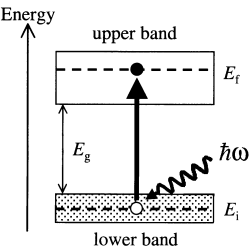
\includegraphics[width=4cm]{../results/intro_energy_absortion.png}
        \caption{}
    \end{subfigure}
    \hfill
    \begin{subfigure}[b]{6cm}
        \centering
        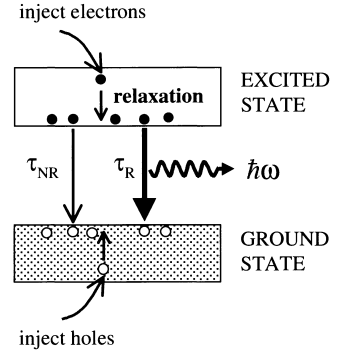
\includegraphics[width=4cm]{../results/intro_energy_emission.png}
        \caption{}
    \end{subfigure}
    \hfill
    \caption{Schematic diagram of (a)light absortion (b)light emission \cite{condensed_matter_optics}}
    \label{fig:pl_intro}
 \end{figure}

 \begin{figure}[ht]
    \centering
    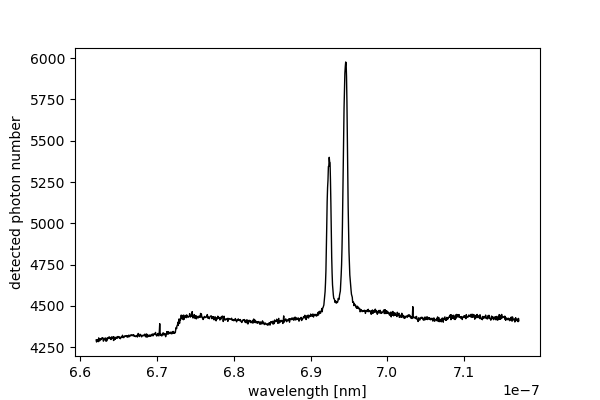
\includegraphics[width=8cm]{../results/Ruby(170.0)_raw_fig.png}
    \caption{photoluminescence results of Ruby in $170.0K$}
    \label{fig:pl_sample}
 \end{figure}
 Fig. \ref{fig:pl_intro}(a) shows the band diagram explaination of light absortion, creating hole in lower band transite to upper band.
 Fig. \ref{fig:pl_intro}(b) is the schematic diagram of light emission, slowly relaxing and emitting light while energy drops between band gap.
 Fig. \ref{fig:pl_sample} is one of the photoluminescence results in this experiment.
 The absorbed light was $532nm$, but we can find out the emitted light have wavelength around $690nm$.
 We can sure the electronic transition is the key mechanisms since the wavelength change can not be explained by scattering, especially for the peak nature.
 Therefore, the peak position is specific to the crystal structure or the molecular shapes.
 But the peak width have two reasons, natural and optical broadening. (\cite{quantum_optics})
 Natural broadening is intrinsic to the transition, caused by lifetime of the states.
 For lifetime $\tau$, the spectral function follows Lorentzian like equation (\ref{equation:natural_broadening}), $\omega$ is the angular frequency of light, and $\Delta \omega$ is full width at half maximum(FWHM) value which is related with lifetime.
 \begin{equation}
   g(\omega) = \frac{\Delta \omega}{2 \pi} \frac{1}{(\omega-\omega_0)^2 + (\Delta \omega/2)^2},\, \Delta \omega = \frac{1}{\tau}
   \label{equation:natural_broadening}
 \end{equation}
 And by the spectral effects by spectroscopy itself, the Gaussian shape optical broadening is inevitable.
 Therefore, I assume that the detected photoluminescence spectroscopy data will follow Voigt profile, which is a convolution results of Lorentzian and Gaussian function.

 \subsection{Ruby}
 \label{intro:ruby}
 In the theory of solid state luminescence, simultaneous emission is allowed between special states.
 Otherwise, electron can loses its energy in phonon which we call nonradiative transition.
 The phonon physics is explained by debye model, assuming that the highest frequency of phonon is restricted by the size of the lattice denoted as $\omega_D$.
 And phonon follows boson statics, can easily induces the density of states.
 
 \begin{multline}
  H= \sum_{n=0}^3 \epsilon_n \psi_n^\dagger \psi_n + \sum_k (\hbar \nu k) (a_k a_k^\dagger + \frac{1}{2}) + S_0 (C_{12} \psi_1^\dagger + \sum_{n=1,2} C_{n3} \psi_n^\dagger \psi_3 + c.c.) \\
   + S_0^2 (\sum_{n=0}^2 d_n \psi_n^\dagger \psi_n + [d_{12}\psi_1^\dagger \psi_2 + c.c.])
  \label{equation:phenomenological_hamiltonian}
 \end{multline}

 In \cite{Ruby_temp_theoretical}, they declare the phenomenological Hamiltonian of impurity ruby as equation \ref{equation:phenomenological_hamiltonian}.
 As the two big peak is observed near $690nm$, we assume three excited-state levels $n=1,2,3$ have energy of $\epsilon_1, \epsilon_2, \epsilon_3$ and wave function of $\psi_1, \psi_2, \psi_3$ respectivly.
 The first term is about the impurity electronic states energy.
 The second term is phonon energy, which $k$ is bounded by Debye frequency.
 In ruby, first and second excited states are $E_2$ levels and the photoluminescence peak appears by the spontaneous emission through $1\rightarrow0$ and $2\rightarrow0$.
 Empirically, $0=\epsilon_0<<\epsilon_1 < \epsilon_2 << \epsilon_3$, since the gren laser excites electron by $0\rightarrow3$ and by nonradiative $3\rightarrow1,2$ transition occurs.
 The leftover terms are suggested perturbation term in \cite{Ruby_temp_theoretical}, assuming the dopped $Cr^{3+}$ locates isotropic in enlarged Debye-model.
 In this experiment, the dopped ratio is small enough to fit in the assumption.
 \begin{multline}
  \epsilon_n (T) = \epsilon_n (0) + \alpha_n (\frac{T}{T_D})^4 \int_{0}^{T_D / T} dx \frac{x^3}{e^x -1} - \beta_{12} (-1)^n \frac{T_e}{T_D} (\frac{T}{T_D})^2 \\
  \times \int^{T_D/T}_{0} dx \frac{x^3}{e^x -1} \frac{P}{x^2 - (T_e/T_D)^2}
  \label{equation:peak_position}
 \end{multline}
 \begin{multline}
  \Gamma_n(T) = \Gamma_n(0) + \bar{\alpha_n} (\frac{T}{T_D})^7 \int^{T_D/T}_{0} dx \frac{x^6 e^x}{(e^x -1)^2}\\ + \pi \beta_{12} (\frac{T_e}{T_D})^3 [\delta_{n2}+\frac{1}{e^{T_e/T}-1}]
  \label{equation:peak_width}
 \end{multline}
 After calculating lowest order of perturbation theory, we have the peak position in function of temperature as equation \ref{equation:peak_position}.
 $T_D$ is Debye temperature, $\alpha_n , \beta_{12}$ is fitting coefficients, $T_e=(\epsilon_2 - \epsilon_1)/k_B$ is $42K$ in ruby.
 Equation \ref{equation:peak_width} shows the temperature dependance of each peak width, $\Gamma$ denotes the parameter of Lorentzian lineshape.
 $\bar{\alpha_n}$ is also a fitting variable, which have direct expression to hamiltonian coefficients.
 The first temperature perturbed term starting with $\alpha_n, \bar{\alpha_n}$ in both equation is a calculation of nonradiative effects.
 The second term starting with $\beta_{12}$ is the term of internal conversion between state $1,2$.
 In this case, the internal conversion can be disregarded, $\beta_{12}=0$.
 Specific fitting method and results in this experiment are denoted below. (\ref{result:temperature_peak_statics})

 Those explaination doesn't imply the specific states, since we never comes out with the crystal environments.
 Ruby is dopped crystal which basic structure is built by $Al_2O_3$, hexagonal crystal structure, $Cr^{3+}$ located in octahedral site.
 In this case both crystal and ion energy state affect themselves to have broad band structure or energy splits.
 $Al_2 O_3$ doesn't have any fluorescence bandgaps, since we can never find photoluminescence peaks on other dopped ions.
 Which means that the affected $Cr^{3+}$ energy structure is the key of this luminescence effects.
 Fig \ref{fig:ruby_band_structure}, adapted from \cite{Ruby_band_structure} shows the shift of ioninc energy structure.
 The left side of the diagram is the original orbital energy of free $Cr^{3+}$.
 As the cubic field parameter $Dq/B$ increases, the energy level splitted and broadened.
 The diagram at $Dq/B=3$ represents energy level of the $Cr^{3+}$ in ruby, which doesn't splitted enough and considered as constant.
 So, $^4A_2 , ^2E, ^2T_1 , ^4T_2$ is the $\epsilon_0, \epsilon_1, \epsilon_2, \epsilon_3$ state respectivly as explained.
 As a conclusion, the dopped ruby absorb green light to transite electron from $^4A_2 \rightarrow ^4T_2$ and nonradiative transite to $^4T_2 \rightarrow ^2T_1 , ^2E$ and give $R_1 , R_2$ emitted light peak by $^2T_1 , ^2E \rightarrow ^4A_2$. 

 \begin{figure}[ht]
  \centering
  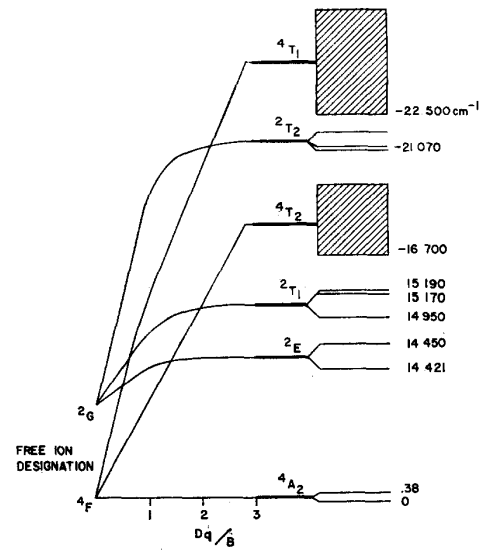
\includegraphics[width=6cm]{../results/ruby_band_diagram.png}
  \caption{Energy level diagram of $Cr^{3+}$ in ruby. adapted form \cite{Ruby_band_structure}}
  \label{fig:ruby_band_structure}
\end{figure}


\subsection{Rhodamine 590(R590)}
 principle of lasers 88p. Frank condon principle.
 In photochemistry the nonradiative, and radiative transition can be explained once in Jablonski diagram.
 Jablonski diagram have each vibrational modes in multiplicity of states, denoted by $M = 2S+1$. $S$ is total electric spin.
 For example, if the all electron is in spin pair, $S=0 , M=1$.
 It is singlet state.
 By the value of $M=1,2,3,4, ... $ the state will named after singlet, doublet, triplet and so on.
 The state $^4S$ is fourth excited state of singlet.

\section{Methods}

\section{Results and Discussion}
\subsection{photoluminescence result fitting method}
\label{result:iris_effect}

\subsection{Ruby PL result by temperature}
\label{result:temperature_peak_statics}



\section{Summary}

\bibliography{photoluminescence_ref}
\bibliographystyle{plain}
\end{document}